%%%%%%%%%%%%%%%%%%%%%%%%%%%%%%%%%%%%%%%%%%%%%%%%%%%%%%%%%%%%%


%Our approach was built around domain specific languages defined using \textit{EMF} (Eclipse Modeling Framework) and \textit{XText}, with execution semantics implemented in \textit{ALE} \cite{leduc01}.

%We take as input the syntax and the semantics of a language defined using the visitor pattern, and give as output a generated language specialized for REPL execution (Figure~\ref{fig:overview}).

%This new language defines an Interpreter entry-point, that manages the context and drives the execution from the top-level, and also outlines the different instructions that will become the interactive entry-points.

%A wrapper for the \textit{ALE} execution engine (Figure~\ref{fig:engine-wrapper}) takes care of creating the \textit{Interpreter} and initializing it.
%It then parses the user input into an actual executable instruction and sets it as the current instruction of the interpreter before executing it.

%The scope of previous instructions is kept by a linked list structure in the current one.
%A custom scope provider uses it for cross references resolution.

%It is important to note that we do not support adding new rules to the concrete syntax of the base language.
%Also, we decided to use the existing grammar rules as the granularity for parsing.
%The consequence is that any instruction that could not be parsed by a rule of the base language will not be supported by the REPL language.

%As for the semantics, the instruction rules need to be executable individually, which means that instructions need to either own their complete context, or use dynamic data defined globally during the initialization of the interpreter.
%If the context cannot be properly initialized on its own, we still give the ability to a language designer to include custom rules in the semantics, but we do not try to infer them during the REPL language generation.

\section{Technical Details and Implementation}
\label{transformation}

This section describes the technical details of the different steps of our approach, and proposes a particular implementation\footnote{See our prototype at \url{https://anonymous.4open.science/r/84105ce9-f47c-4dd2-936e-9eb2dd345ad0/}}. 

The proposed implementation comes in the form of a prototype based on the GEMOC Studio \cite{bousse:hal-01355391}. The GEMOC Studio is an Eclipse package on top of the Eclipse Modeling Framework \cite{steinberg2008emf}, which has been experienced in various industrial projects. Among others, it offers a language workbench that supports the modular specification of DSLs, using Ecore for the abstract syntax, Xtext for the textual concrete syntax, OCL or Xtend for the static semantics and ALE for operational semantics. Other alternatives are also proposed but not illustrated in the scope of this paper. 

We illustrate both the approach and the implementation using the simple but real-world \emph{Logo} language introduced in Section \ref{motiv}. 

\begin{comment}

\subsection{Technological environment}

In order to define the approach in practice, we have chosen to set up a technical stack. The Gemoc studio was chosen for three main reasons: \textsc{i)} The underlying technologies are used industrially. It is an environment that requires a good separation between both \textsc{ii)} the grammar definition and the AST nodes definition and \textsc{iii)} the specification of the different static and operational semantics. The language workbench uses object oriented technologies for representing the AST and the interpreter pattern for specifying the operational semantics. 

The GEMOC Studio provides generic components through Eclipse technologies for the development, integration, and use of heterogeneous executable modeling languages. This includes, among others:

\begin{itemize}
    \item metaprogramming approaches and associated execution engines to design and execute the behavioral semantics of executable modeling languages,
    \item efficient and domain-specific execution trace management services and model animation services,
    \item advanced debugging facilities such as forward and backward debugging (i.e. omniscient debugging), timeline, etc.
    \item coordination facilities to support concurrent and coordinated execution of heterogeneous models,
    \item an extensible framework for easily adding new execution engines and runtime services.
\end{itemize}

\end{comment}

\subsection{DSL Specification Enhancement}\label{sec:v2rmetamodel}

As presented in Section~\ref{approach}, we first provide to the language engineer the relevant abstractions for specifying the multiple execution entry-points:
\begin{itemize}
    \item Identification of the valid instructions to be executed independently,
    \item Definition of the expected outputs as intermediate results, and
    \item Definition of the help messages for the language user. 
\end{itemize}

In practice, these information could be provided either in the syntax or in the semantics. However, we had to consider that the visitor can be augmented by additional helpers for a given Ecore object, and there is no way of deciding on which to use. Besides, the output needs to refer to dynamic information which is mainly available within the semantics. %Thus, metadata required for the REPL is bound with the AST nodes and the associated operational semantics. 

In order to identify the required entry-points, the language designer could methodically:
\begin{enumerate}
  \item take a look at each rule of the grammar and choose the ones to provide in the REPL
  \item decide on the expected outputs for each of the chosen rules
  \item factor them in to abstract parent rules if the outputs are the same
\end{enumerate}

To let the language engineer define the required information, we introduce a new metamodel shown in Fig.\ref{fig:ReplDefinitionMetamodel}. It can be seen as a dedicated meta-language to modularly complement the initial DSL specification with information related to the REPL. The core element of this metamodel is the \textit{Instruction} meta-class. It defines three main information required to generate the REPL:
\begin{enumerate}
   \item the new entry point in referencing a specific AST and the ALE method that defined the operational semantics for this node.  
  \item the help message to display if a user wishes to request help on this specific entry point.
  \item the elements of the semantics to be used as textual outputs of the interpreter. These elements can be either attributes related to the execution (\emph{i.e.,} attributes of the operational semantics), calls to existing methods of these semantics, or calls to ALE methods defined by the language engineer (\emph{e.g.,} \textit{evalResult} and a set of \textit{evalParams} that could target an \textit{ALE Expression}).
\end{enumerate}

The second main meta-class is \textit{Interpreter}. It allows language engineers to specialize, among other things, the initialization of the execution context of the interpreter. 

\begin{figure*}[t]
	\centering
	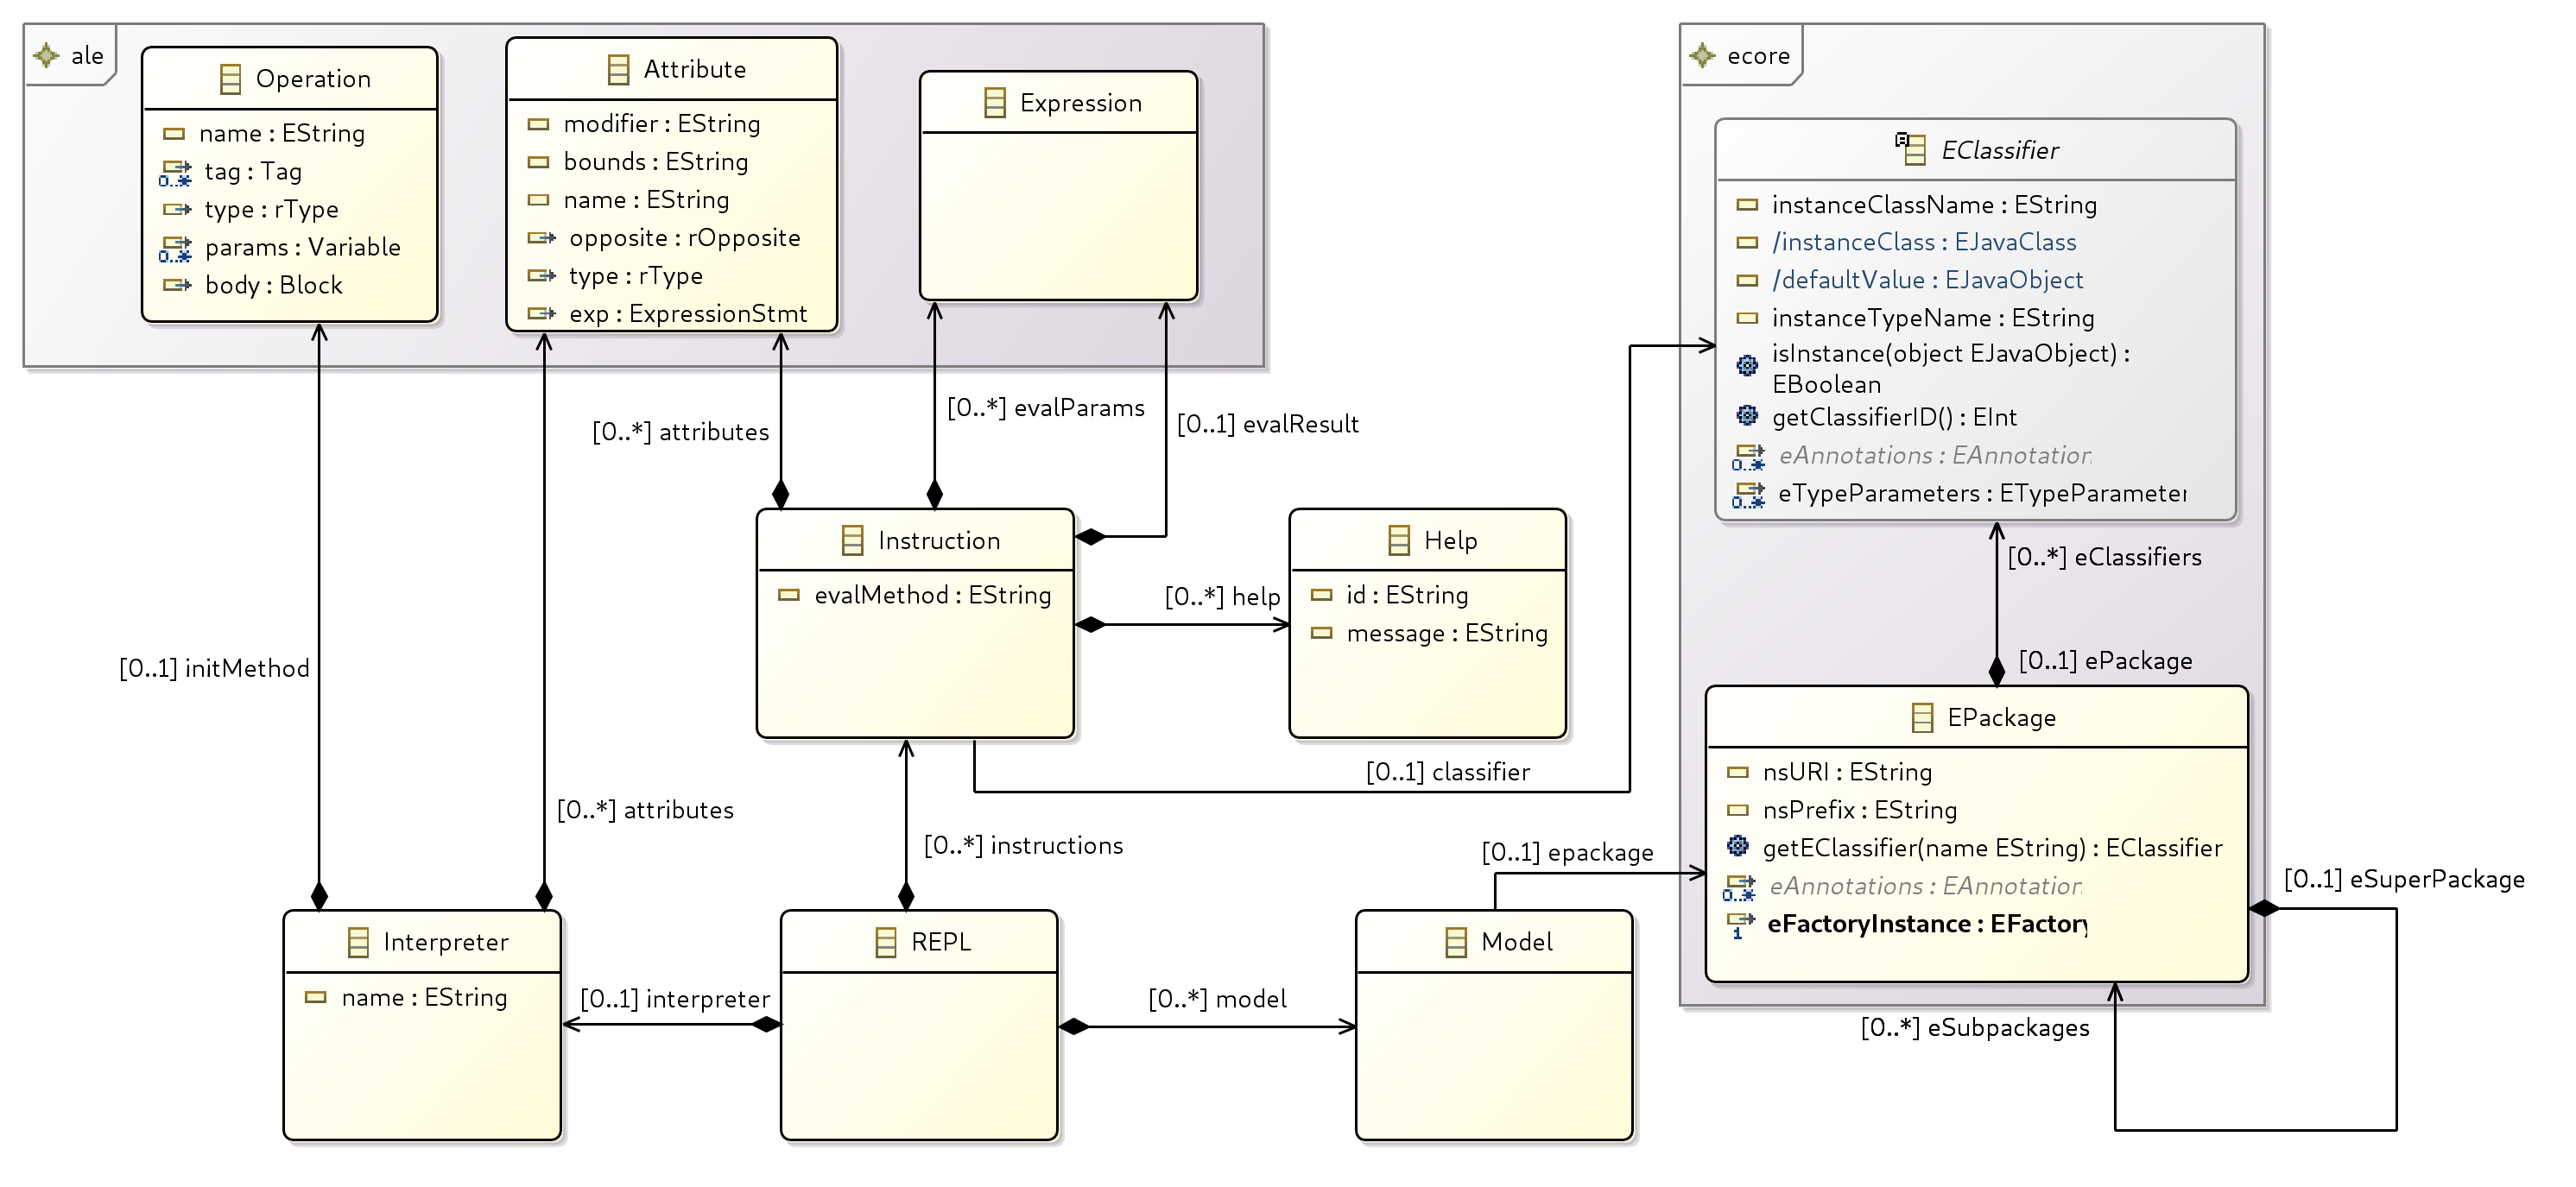
\includegraphics[width=.95\linewidth]{figures/visitor2repl_class_diagram.png}
	\caption{ReplDefinition metamodel}
	\label{fig:ReplDefinitionMetamodel}
\end{figure*}

We provide two concrete syntax to populate the model conform to the \textit{ReplDefinition} metamodel: a dedicated DSL, and additional annotations to ALE. This model represents the required information to drive the transformation of the DSL specification. 

\paragraph{Using a new DSL:}

The first concrete syntax is a new DSL built as an extension of ALE. Fig.~\ref{fig:repltransfo} shows the definition of the REPL for the \emph{Logo} language. 

The first part defines the entry points, associated outputs and help messages.  It defines two new entry points: Statement::execute and Expression::compute. It also defines their associated outputs to display: \textit{logo\_repl.turtle.toString()} and \textit{output.toString()} (\textit{output} refers to the actual value possibly returned by the entry-point). Finally we could define the help associated with these entry points (it has been done only partially in the Logo example). % \todo{ca serait bien de donner un example ici}

The second part specifies the \textit{Interpreter}, the specialization of its context of execution and its initialization.   
\textit{Interpreter} will serve as the starting point of the execution of the REPL and will manage the future instructions.
It will contain the same kind of runtime data as the entry-point of the base DSL, which will define the global context of the REPL. In the case of \textit{Logo}, this means the turtle graphics, and a symbol table used to define procedures (using a symbol table for this is simply a design choice of the language engineer). In order to initialize this global context, the initialization method of the interpreter will also be the same as the base DSL.

%In the current case, it defines a new execution context with two attributes \textit{Turtle} and \textit{SymbolTable} and defines their setup. These types exist in the current operational semantics. 

\begin{figure}[t]
	\centering
	\lstset{%
	    basicstyle=\scriptsize,
	    frame=single,
	    morekeywords={extend, as, interpreter, attribute, initmethod, instruction, output, help},
	    emph={syntaxmetamodel},
	    emphstyle=\itshape
	}
\begin{lstlisting}
extend http://www.gemoc.org/logo as logo

instruction logo.Statement:
    help right "Turn turtle of 'p' degrees to the right" 
    help forward "Move turtle of 'p' units forward" 
    execute(logo_interpreter.turtle, logo_interpreter.st)
        => logo_interpreter.turtle.toString();
instruction logo.Expression:
    compute(logo_interpreter.st)
        => output.toString();

interpreter logo_interpreter {
    attribute Turtle turtle;
    attribute SymbolTable st;
    initmethod def void init() {
        self.turtle := Turtle.create();
        self.turtle.xpos := 0.0;
        /* ... */
        self.st := SymbolTable.create();
        self.st.init();
    }
}

	\end{lstlisting}
	\caption{Example of ReplDefinition model for Logo}
	\label{fig:repltransfo}
\end{figure}

%As such, we chose to include them in the semantics, directly on the right operation.
\paragraph{Using annotations}

The same kind of information can be defined directly within the existing ALE operational semantics using a set of annotations.  We provided the language engineer with the following annotation:
\begin{alltt}
    @repl\textcolor{gray}{__outputtarget}\textcolor{lightgray}{__outputcall__...}
\end{alltt}
The output specification here is optional, and represents either an attribute read or a method call on a semantic object from the global context, or on the result of the operation being annotated. Note that the syntax is based on underscores because of limitations of the ALE language, which only supports identifiers as annotations.
Using two underscores as the separator allows for compatibility with semanics using either camel case or snake case for identifiers.

The language engineer can also set the help message to display by using a \textit{javadoc} like comment:
\begin{alltt}
    \textcolor{gray}{/**
     * keyword: Help message
     */}
\end{alltt}

In the base semantics for \textit{Logo}, the only additions besides the optional help messages were the two following annotations (cf. Github repository):
\begin{itemize}
    \item \verb|@repl_turtle_toString| for the \verb|execute| operation of \textit{Statement}
    \item \verb|@repl_output_toString| for the \verb|compute| operation of \textit{Expression}
\end{itemize}


\begin{figure}[t]
	\centering
	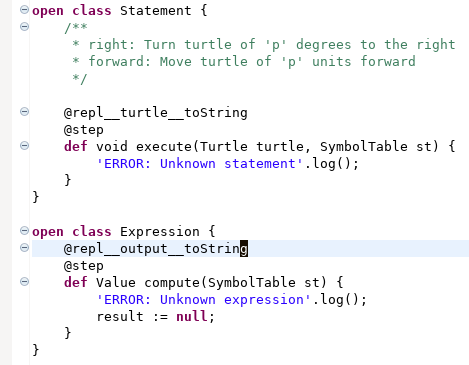
\includegraphics[width=\linewidth]{figures/annotations.png}
	\caption{ReplDefinition annotations used on Logo language}
	\label{fig:ReplDefinitionAnnotation}
\end{figure}

Fig~\ref{fig:ReplDefinitionAnnotation} shows a code excerpt from the operational semantics of the Logo language extended with the proposed annotations to define the information required to complement the DSL specification with an interactive programming environment. The set of annotations is however less expressive than the DSL. Indeed a language engineer might want to use a more complex expression as the output of an instruction or specialize the execution context for the REPL, which could not be done through annotations.
One could still choose to modify the behavior of the base semantics by adding a new ALE operation that could then contain any kind of ALE expression, and call it in the annotation.
This new operation could not, however, have access to the global context of the interpreter, nor to the intermediary results.

Based on this information, the DSL specification can be transformed so that a REPL can be derived and used by interactive computer programming environments. It is defined in three steps \textsc{i)} Abstract Syntax Tree transformation, \textsc{ii)} Concrete Syntax transformation, \textsc{iii)} Operational semantics transformation. The next subsections detail these three transformations applied on the original DSL specification. Finally, we present the generic REPL interface provided and the clients defined as interactive computer programming environments: a language shell and a notebook interface. 

%For this reason, we start by generating an intermediary transformation model written with a custom DSL (\textit{V2R}) that is openly editable (even though this is not necessary to obtain a working REPL).

%\subsection{V2R transformation model}



%\subsection{Grammar specification transformation}

%Using the annotated semantic and the definition of the abstract syntax, our tool generates a transformation model that defines all the mappings between the two languages.

%An example can be seen in figure~\ref{fig:v2r} with the language \textit{Logo}.


%Next are the instructions.
%For each \textit{repl} annotation from the semantic, the transformation model will include a mapping between the annotated method, actual parameters found from the runtime data of the interpreter, and optionally the expected outputs as defined in the annotation.

\subsection{Abstract syntax transformation}

\begin{figure}[t]
	\centering
	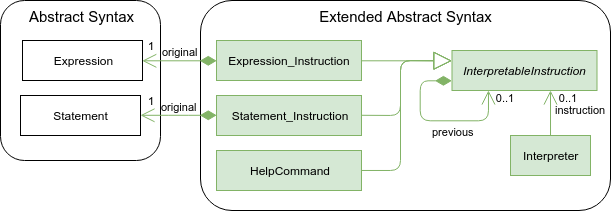
\includegraphics[width=\linewidth]{figures/sle_abstract_syntax.png}
	\caption{Abstract Syntax extension for Logo}
	\label{fig:as}
\end{figure}

During the DSL specification transformation process, we first complement the abstract syntax with additional concepts.

We first define \textit{Interpreter} as the REPL entry-point. It owns a reference to the abstract class \textit{InterpretableInstruction} which will be set during the execution to always target the current instruction.

\textit{InterpretableInstruction} also has a containment to itself, which creates a linked list of the previously executed instructions, hence keeping the whole execution history in a single resource.
For each instruction \textit{I} defined in the \emph{ReplDefinition} model, the new abstract syntax will include an adapter \textit{I\_Instruction} extending \textit{InterpretableInstruction}.
Another instruction is the \textit{HelpCommand}.

An example of the additions made for \textit{Logo} can be seen in Fig.~\ref{fig:as}.
The instructions that correspond to the new entry-points are \textit{Statement} and \textit{Expression}.

\subsection{Concrete syntax transformation}

The second step in our approach is to extend the existing concrete syntax to parse alternatives corresponding to the newly defined instructions.
As such, for each instruction \textit{I}, we retrieve the corresponding rule from the base grammar of the DSL and we reuse it for the newly defined adapter \textit{I\_Instruction}.
The parsing rule \textit{InterpretableInstruction} manages this part.

Another rule is created in order to instantiate an interpreter.
Then, the grammar entry-point will be the parsing rule \textit{EntryPoint} that will call either \textit{Interpreter}, \textit{InterpretableInstruction} or \textit{HelpCommand} if the user asks for help on a specific subject.

We also add a custom scope provider in order to resolve the cross references between the previously executed instructions and the current one.
When trying to resolve a cross reference, this scope provider will browse through the linked list of the previous instructions.
If nothing was found, it will finally turn to the resolution mechanisms of the base grammar.

One of the limitations of this specific implementation is that we use the default Xtext parser to parse single statements.
As such, we do not support non context-free grammars.
If the language has two semantically different instructions that use the same notation, only one of them can be made into an entry-point.
Some possible ways to support non context-free grammars would be:
\begin{itemize}
  \item to use a custom parser that could build a context from the previously executed instruction (which might add unwanted side effects)
  \item or to allow the language designer to modify the keywords used by some grammar rules, in order to remove potential conflicts
\end{itemize}

Fig.~\ref{fig:cs} depicts an organization of the different artifacts related to the concrete syntax extension of the language \textit{Logo}, while Fig.~\ref{fig:ecs} details the corresponding Xtext production rules.

\begin{figure}[t]
	\centering
	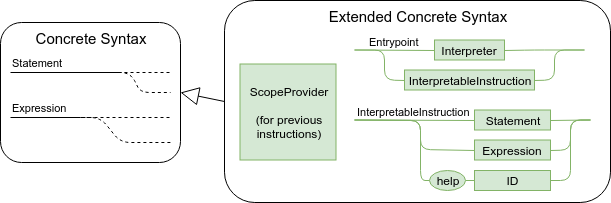
\includegraphics[width=\linewidth]{figures/sle_concrete_syntax.png}
	\caption{Concrete Syntax extension for Logo}
	\label{fig:cs}
\end{figure}

\begin{figure}[t]
	\centering
	\lstset{%
	    basicstyle=\scriptsize,
	    frame=single,
	    morekeywords={returns, repl, attribute, initrepl, instruction, output},
	    emph={syntaxmetamodel},
	    emphstyle=\itshape
	}
\begin{lstlisting}
// Import existing Logo definition. 

EntryPoint returns ecore::EObject:
  InterpretableInstruction | Interpreter;

InterpretableInstruction:
  {Statement_Instruction} original=Statement
    | {Expression_Instruction} original=Expression
    | {HelpCommand} 'help' command=ID;
  
Interpreter:
  {Interpreter}
	\end{lstlisting}
	\caption{Generated extended grammar definition for Logo}
	\label{fig:ecs}
\end{figure}



\subsection{Semantics transformation}

Last, we transform the DSL semantics to incorporate the new execution context and flow management, and to enable the new instructions to be executed.

Here, we handle operational semantics written in ALE.
ALE is a language that allows to re-open classes from Ecore metamodels to statically introduce fields and operations at design time.
By using the \textit{open class} syntax, we can define the behavior for the classes we added in the syntax, and drive the execution with \textit{@init} and \textit{@main} annotations on operations.

We define the runtime data of the execution context and the initialization of the \textit{Interpreter} entry-point as described in the \emph{ReplDefinition} model.
When executed, the interpreter will call the operation \verb|interpret| on the instruction it is currently referencing.

Every instruction adapter takes care of the mapping defined in the \textit{ReplDefinition} model: they become a wrapper that will call the original execution method of the statement or expression, possibly with the right parameters (the interpreter's execution context) and retrieve and display the expected outputs as described in the model.

Fig.~\ref{fig:sem} describes the overall execution flow for the language \textit{Logo}, while Fig.~\ref{fig:esementics} shows the generated ALE code corresponding to this execution flow. The Interpreter, its initialization method and specialized execution context are derived from the information provided by the language engineer in the \emph{ReplDefinition} model (see section \ref{sec:v2rmetamodel}). For each new entry point, an operation is added to manage the semantics. A new operation is also added to the new \textit{HelpCommand} meta-class. 

\begin{figure}[t]
	\centering
	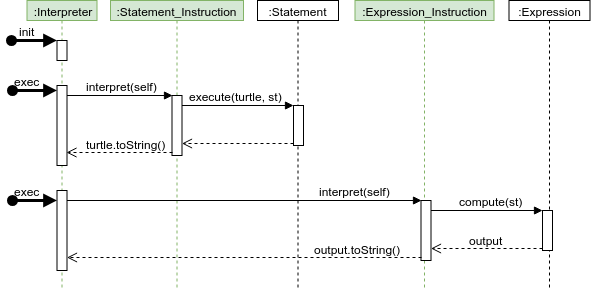
\includegraphics[width=\linewidth]{figures/sle_semantics.png}
	\caption{Overall execution flow for Logo}
	\label{fig:sem}
\end{figure}

\begin{figure}[t]
	\centering
	\lstset{%
	    basicstyle=\scriptsize,
	    frame=single,
	    morekeywords={returns, class, @init, @main,  open, void, def},
	    emph={syntaxmetamodel},
	    emphstyle=\itshape
	}
\begin{lstlisting}
open class Interpreter {
  logolang::Turtle turtle;
  logolang::SymbolTable st;

  @init
  def void init() {
    self.turtle := logolang::Turtle.create();
    self.turtle.xpos := 0.0;
    self.turtle.ypos := 0.0;
    self.turtle.direction := 0.0;
    self.turtle.pendown := false;
    self.turtle.canvas := logolang::Canvas.create();
    self.turtle.canvas.segments := Sequence{};
    self.st := logolang::SymbolTable.create();
    self.st.init();
  }

  @main
  def void run () {
    self.instruction.interpret(self);
  }
}

open class Expression_Instruction {
  def void interpret(Interpreter logo_repl) {
    ecore::EObject output := 
      self.original.compute(logo_repl.st);
    output.toString()?.log();
  }  
}

open class Statement_Instruction {
  def void interpret(Interpreter logo_repl) {
    self.original.execute(logo_repl.turtle, logo_repl.st);
    logo_repl.turtle.toString()?.log();
  }
}

open class HelpCommand {
  def void interpret(Interpreter logo_repl) {
    // Call help method of the node
  }
}

	\end{lstlisting}
	\caption{Generated extended operational semantics for Logo}
	\label{fig:esementics}
\end{figure}


\subsection{REPL Interface and Interactive Environments Examples}

%%%% BEGIN: FROM SECTION 3 %%%%

\begin{figure}[t]
	\centering
	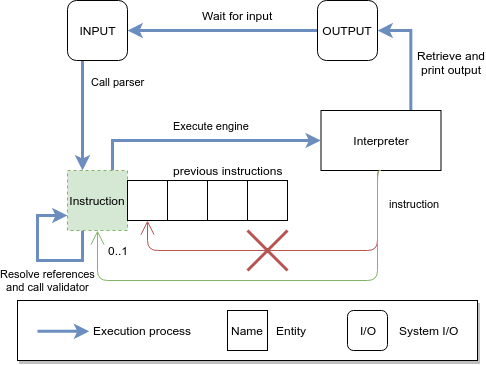
\includegraphics[width=0.9\linewidth]{figures/sle_engine_wrapper.png}
	\caption{REPL execution}
	\label{fig:engine-wrapper}
\end{figure}

Having applied the aforementioned transformation process, the DSL is complemented with a multi entry points parsing of interpretable instructions. In order to build an interactive environments on top of it, we provide a generic REPL interface protocol and its underlying systematic execution framework (cf. Fig.~\ref{fig:engine-wrapper}):
%The generated REPL semantics is the following:
\begin{samepage}
\begin{enumerate}
    \item Create an interpreter and initialize it
    \item \label{loop} Read the user input
    \item Parse it as an instruction
    \item Retrieve the previous instruction and store it
    \item Swap the instruction of the interpreter for the new one
    \item Run the interpreter
    \item Print the relevant output
    \item Go back to step \ref{loop}
\end{enumerate}
\end{samepage}

%%%% END: FROM SECTION 3 %%%%

\begin{figure}[t]
	\centering
	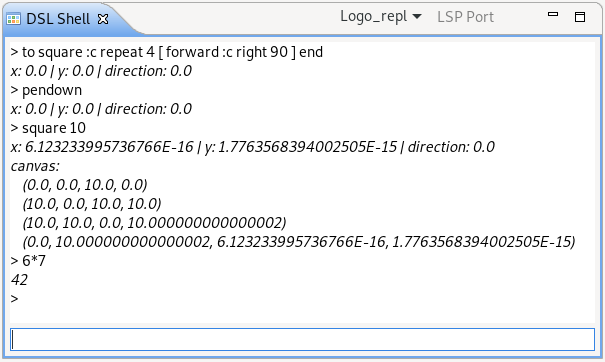
\includegraphics[width=\linewidth]{figures/logo_shell.png}
	\caption{Eclipse shell running with Logo REPL}
	\label{fig:logo_shell}
\end{figure}

From the new generated DSL specification, we automatically generate the entire GLUE code for integration with two technical environments: Eclipse and Jupyter. 
For the first one, we provide a plugin including an eclipse view hosting a shell to communicate with the Interpreter.  This generic view declares an Eclipse extension point type including among others the name of the REPL language and the qualified name of the interpreter class. 
Each REPL language declares this extension point. The generic view allows REPL users to select the desired DSL and then start an interactive session. This session keeps track of the executed instructions and offers the ability to reset the interpreter or cancel the last instructions thanks to the environment provided by Gemoc. The Language Server Protocol (LSP\footnote{\url{https://langserver.org/}}) support provided by Xtext enables intelligent completion within the Shell. Figure~\ref{fig:logo_shell} shows a screenshot of this integration within Eclipse for the Logo language. 

For Jupyter, an editor specific to ipynb files (Jupyter notebook) has been created and manually integrated into Jupyter. The purpose of this editor is to replace the default code cell editor (ace editor\footnote{Cf. \url{https://ace.c9.io/}}) with the monaco text editor\footnote{Cf. \url{https://microsoft.github.io/monaco-editor/}}. The latter has the advantage of natively supporting LSP in order to allow completion, error reporting, etc. A generic glue code has been added to adapt between Jupyter's Kernel concept and GEMOC's execution engine to control the execution of interpreters. Thus for each new REPL, a connection file defining the connection URL to the GEMOC execution engines of this REPL is generated. A descriptor is also generated for Jupyter to register this new kernel. 


\begin{comment}
\begin{figure}[t]
	\centering
\begin{lstlisting}[language=json]
{
 "argv": ["python3", "-m", "REPL.kernel",
          "-f", "{connection_file}"],
 "display_name": "LOGO REPL",
 "language": "logo"
}
\end{lstlisting}
\end{figure}
\end{comment}

On the GEMOC side, a class allowing to interface with a ZeroMQ message oriented middleware is created and makes the link with the execution interface of the GEMOC engine and the current REPL. The main advantages of the GEMOC integration is to leverage its execution trace management, debugging facilities and concurrency model management (e.g., to start from any cell or finely control the flow of execution of the cells.).


%(C'est un peu applatti)
%Les attributs et la méthode init c'est exactement ce que j'ai défini dans le V2R (vu que c'est du ALE de base)
%Et pour le générer dans le V2R, je me suis basé sur l'annotation init de base



%\subsection{REPL Semantics}

%Since we use a regular single-program execution engine, we need to add a mechanism in order to retrieve and reuse the runtime context, in order to get a proper interactive environment.
%It is also necessary to have the read-eval-print-loop behaviour that it lacked.
%As such, we decided to implement this in a wrapper for the base execution engine.

%The first action of this wrapper is to create and initialize the actual engine.
%We consider that the global context for future instructions should be defined during this phase, by calling an initialization method from the semantic.

%Then comes the REPL part: the wrapper manages buffers for both inputs and outputs, and will continuously wait for new input before processing it as intended.
%Having received a new instruction as a string, it parses it to an actual executable instruction by following the rules of the previously generated syntax (Section~\ref{transformation}).
%The input can also be an internally defined command: in our case, we have \textsc{exit} and \textsc{help}.
%If there were previously executed instructions in the current instance, the instruction gets enriched with the whole history.
%Post-parsing operations like cross references resolution and validations are manually applied, then the instruction gets passed to the actual engine with the runtime context (in the case of the ALE engine, the context is kept by the engine as long as we don't manually reset it).
%At last, the wrapper captures the outputs and errors from the whole process and stores them in its buffers.
